% ------------------------------------------------------------------------------
% Your readers must be able to understand at a glance which data set belongs to which research question or hypothesis.
% - Describe your data objectively
% - Use graphs and tables to illustrate your data.
% - Refer to your research question with each result
% - Rank your results in order of importance
% - Confirm or reject your hypotheses
% ------------------------------------------------------------------------------

\opt{never}{\addbibresource{03-tail/bibliography.bib}} % to make citation found in most IDE

\chapter{Validation}
\label{chap:validation}

% -- Your text goes here --
This chapter presents the tests carried out and their results to prove that the reference architecture works in its entirety. The notion of cost at \gls{cloud_infrastructure} level is also addressed. 

\minitoc
\newpage

% -----------------------------------------------------------------------------
\section{Project configuration}

% -- Your text goes here --
Before pushing this reference architecture into a new GitHub repository, a few project configurations have been made. Firstly, it is essential to add the GitHub Actions user as a trusted identity so that \gls{aws} can grant him access to its resources. In the \gls{aws} account on which the infrastructure is deployed, the GitHub identity provider is specified (figure \ref{fig:1_Identity_provider}).
\begin{center}
    \begingroup
    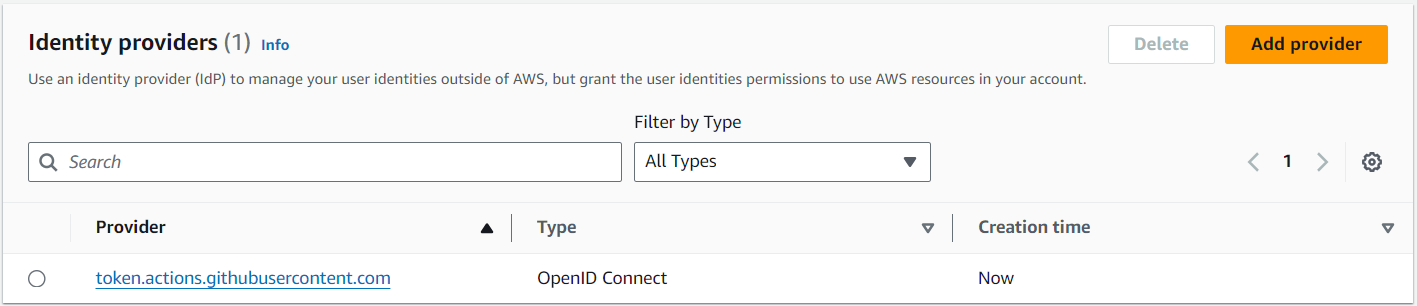
\includegraphics[width=1\columnwidth]{validation/1_Identity_provider.png}
    \captionof{figure}{GitHub identity provider}
    \label{fig:1_Identity_provider}
    \endgroup
\end{center}
An IAM role has been set up to authorise only the project's GitHub repository to access resources. A policy is linked to limit the actions allowed on the resources (figure \ref{fig:2_OIDCRole}).
\begin{center}
    \begingroup
    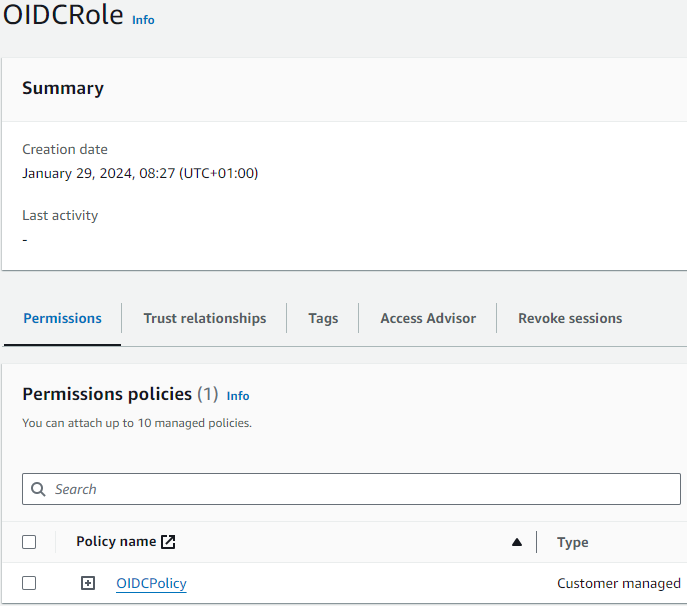
\includegraphics[width=.8\columnwidth]{validation/2_OIDCRole.png}
    \captionof{figure}{IAM OIDC role}
    \label{fig:2_OIDCRole}
    \endgroup
\end{center}
The secret and visible variables that need to be configured have been added to the GitHub repository (figures \ref{fig:3_SecretVar_GitHub} and \ref{fig:3_Var_GitHub}).
\begin{center}
    \begingroup
    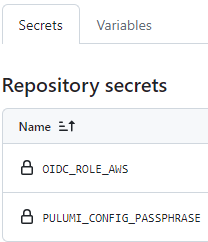
\includegraphics[width=.25\columnwidth]{validation/3_SecretVar_GitHub.png}
    \captionof{figure}{GitHub secret variables}
    \label{fig:3_SecretVar_GitHub}
    \endgroup
\end{center}
\begin{center}
    \begingroup
    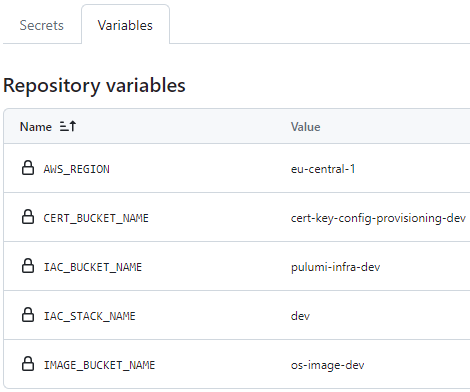
\includegraphics[width=.5\columnwidth]{validation/3_Var_GitHub.png}
    \captionof{figure}{GitHub visible variables}
    \label{fig:3_Var_GitHub}
    \endgroup
\end{center}
The configuration file for the Pulumi tool was configured by specifying the \gls{aws} account ID and the region (figure \ref{fig:4_Set_Pulumi_Stack}).
\begin{center}
    \begingroup
    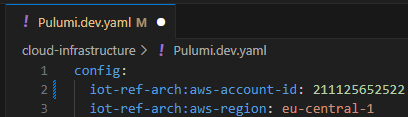
\includegraphics[width=.55\columnwidth]{validation/4_Set_Pulumi_Stack.png}
    \captionof{figure}{Pulumi configuration file (development environment)}
    \label{fig:4_Set_Pulumi_Stack}
    \endgroup
\end{center}
Finally, the serial numbers of the devices authorised to be provisioned have been listed. In this case, only a Raspberry Pi 4 is authorised (figure \ref{fig:5_Set_Allowlist}).
\begin{center}
    \begingroup
    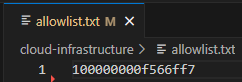
\includegraphics[width=.3\columnwidth]{validation/5_Set_Allowlist.png}
    \captionof{figure}{Embedded systems allowlist}
    \label{fig:5_Set_Allowlist}
    \endgroup
\end{center}

\section{\texorpdfstring{\acrshort{ci}/\acrshort{cd}}{} pipeline}

% -- Your text goes here --
After the previous configuration, the project was pushed into the GitHub repository. The \acrshort{ci}/\acrshort{cd} pipeline started automatically, beginning with the deployment of the \gls{cloud_infrastructure}. All tasks were completed successfully. The different times for each workflow can be seen on the right-hand side of figure \ref{fig:6_Workflows}. Total process time is just over 10 minutes.
\begin{center}
    \begingroup
    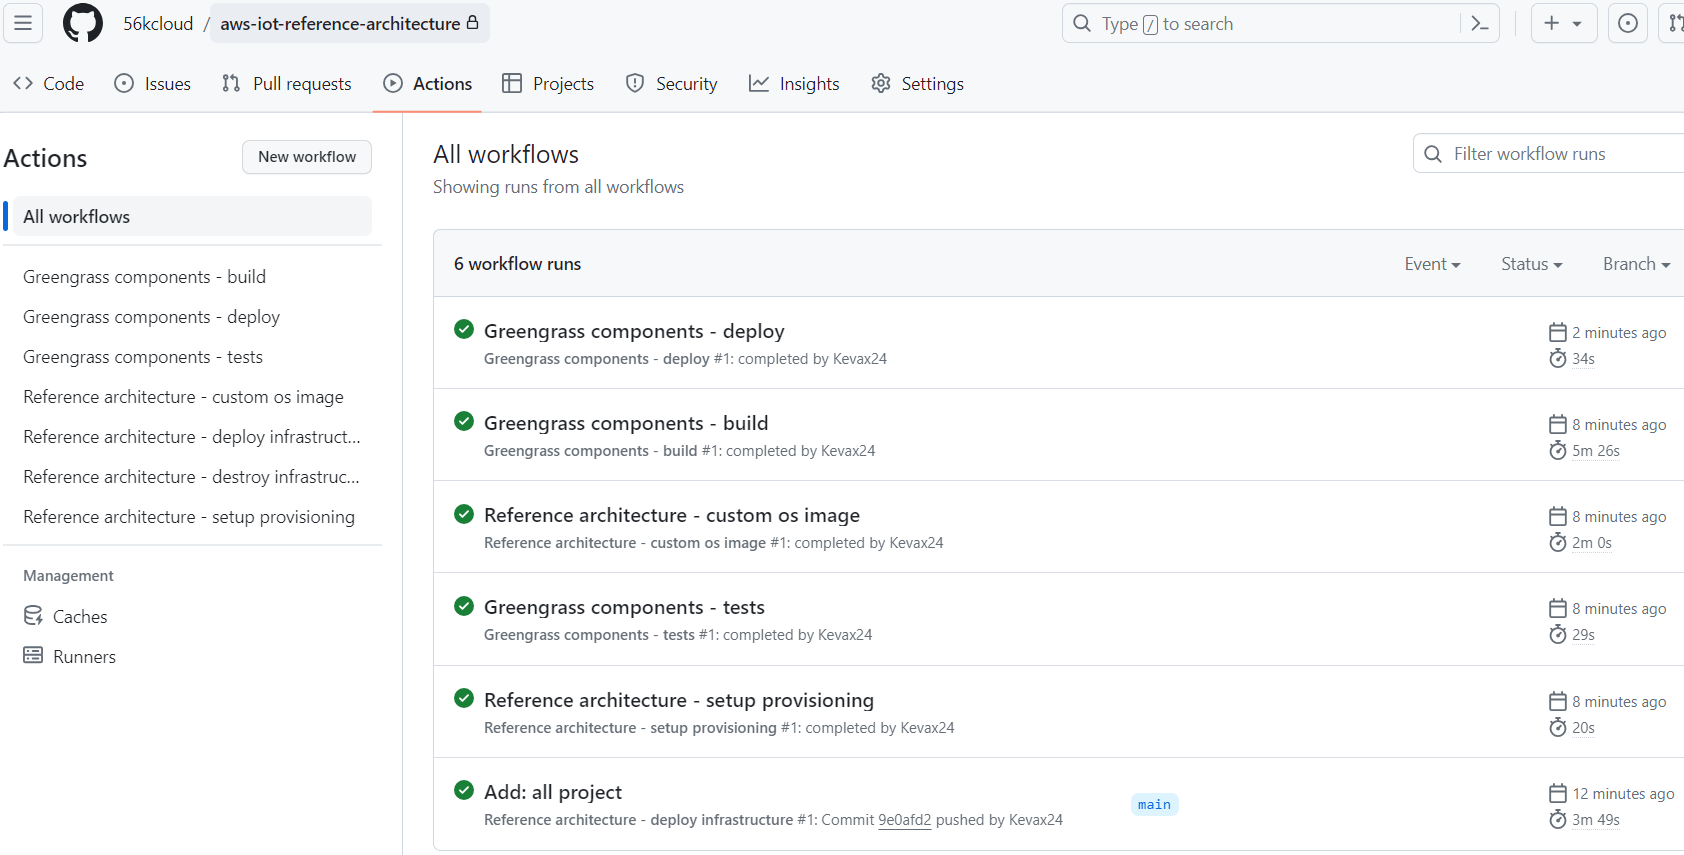
\includegraphics[width=1\columnwidth]{validation/6_Workflows.png}
    \captionof{figure}{Successful workflows}
    \label{fig:6_Workflows}
    \endgroup
\end{center}
The \gls{cloud_infrastructure} has been deployed on the development account specified and in the \textit{eu-central-1} region. The configuration for the provisioning of the embedded systems was carried out correctly with the creation of the \acrshort{os} image. The base image used is \textit{Raspberry Pi \acrshort{os} Lite} based on the Debian distribution.

At the same time, the applications were tested, including the led application, the button application and the certificate rotation application. Five Greengrass components were created and published in \gls{aws}. These components were also deployed.

\section{\texorpdfstring{\Gls{cloud_infrastructure}}{} deployment}

% -- Your text goes here --
All the resources described in Pulumi have been created correctly. In this sequel, they are not all mentioned and presented in images due to the sheer number of resources. An example is shown in figure \ref{fig:10_Infra_S3} where the S3 buckets have been created. There is the storage space for the state of the infrastructure, another for the provisioning configuration and finally one where the \acrshort{os} image is stored.
\begin{center}
    \begingroup
    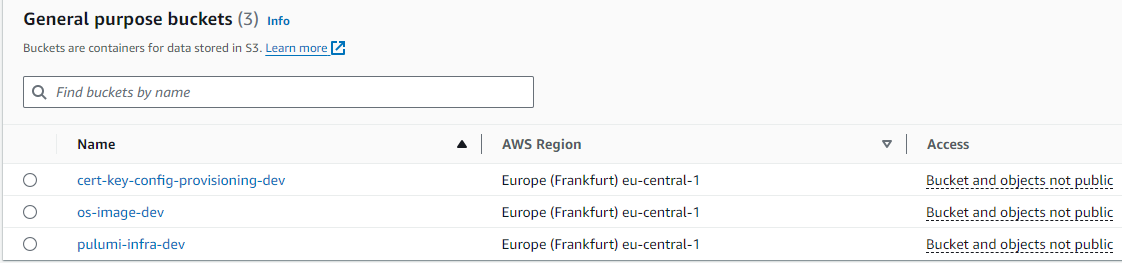
\includegraphics[width=1\columnwidth]{validation/10_Infra_S3.png}
    \captionof{figure}{S3 buckets}
    \label{fig:10_Infra_S3}
    \endgroup
\end{center}
The \acrshort{iot} device group has been created under the \textit{GreengrassGroup} name. Two policies were created for \gls{provisioning} and for interactions once provisioned (figure \ref{fig:10_Infra_IoT_Policies}). The claim certificate has also been prepared and linked to the \gls{provisioning} policy.
\begin{center}
    \begingroup
    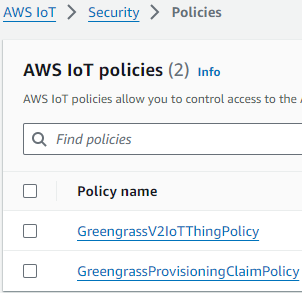
\includegraphics[width=.3\columnwidth]{validation/10_Infra_IoT_Policies.png}
    \captionof{figure}{\acrshort{iot} policies}
    \label{fig:10_Infra_IoT_Policies}
    \endgroup
\end{center}
The Greengrass components have been successfully published (figure \ref{fig:10_Infra_IoT_Components}). Docker images of the applications are also available in the Amazon \acrshort{ecr} service.
\begin{center}
    \begingroup
    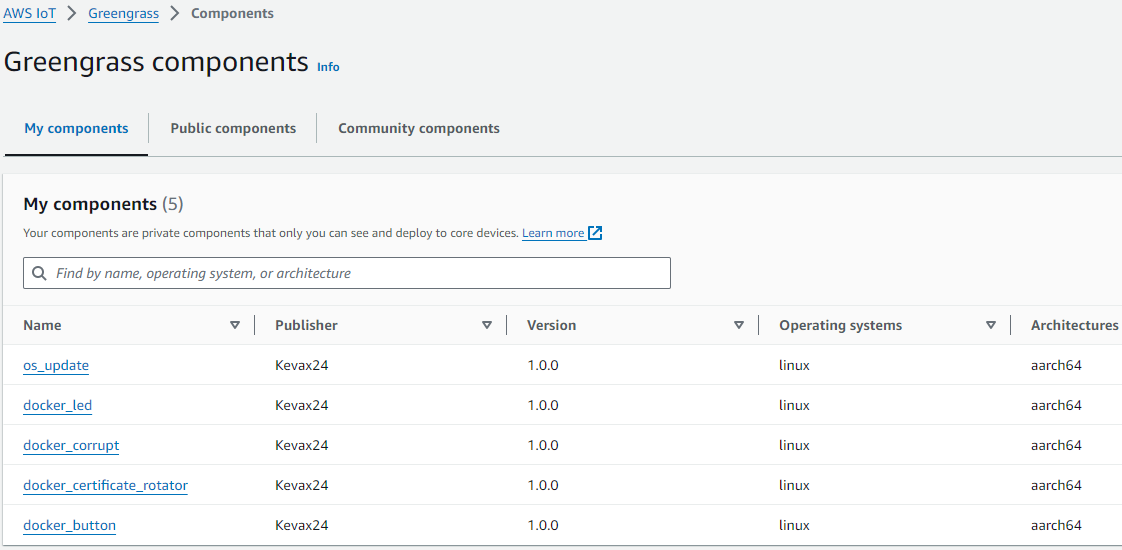
\includegraphics[width=1\columnwidth]{validation/10_Infra_IoT_Components.png}
    \captionof{figure}{Greengrass components}
    \label{fig:10_Infra_IoT_Components}
    \endgroup
\end{center}
A deployment service is ready to deploy applications as soon as devices are provisioned. It targets the group created (figure \ref{fig:10_Infra_IoT_Deployment}).
\begin{center}
    \begingroup
    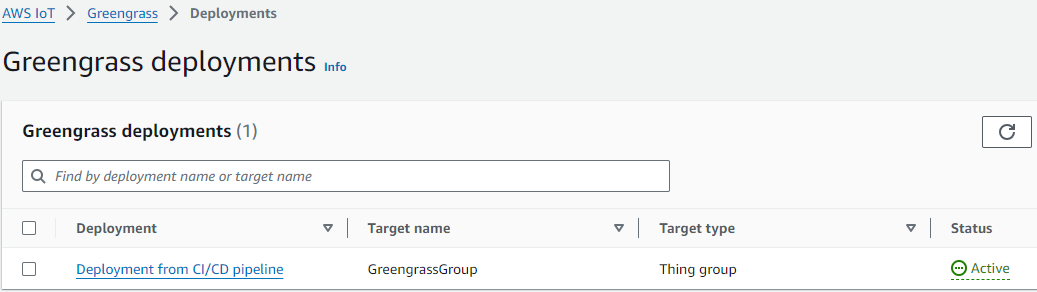
\includegraphics[width=1\columnwidth]{validation/10_Infra_IoT_Deployment.png}
    \captionof{figure}{\gls{aws} \acrshort{iot} Greengrass Deployment}
    \label{fig:10_Infra_IoT_Deployment}
    \endgroup
\end{center}

\section{\texorpdfstring{\Gls{provisioning}}{} a Raspberry Pi 4}

% -- Your text goes here --
The integration of an \acrshort{iot} device was a success. A Raspberry Pi 4 was provisioned. The \acrshort{os} image was first downloaded from the S3 bucket. It was then flashed into an SD card (figure \ref{fig:7_Flashing_SDCard}).
\begin{center}
    \begingroup
    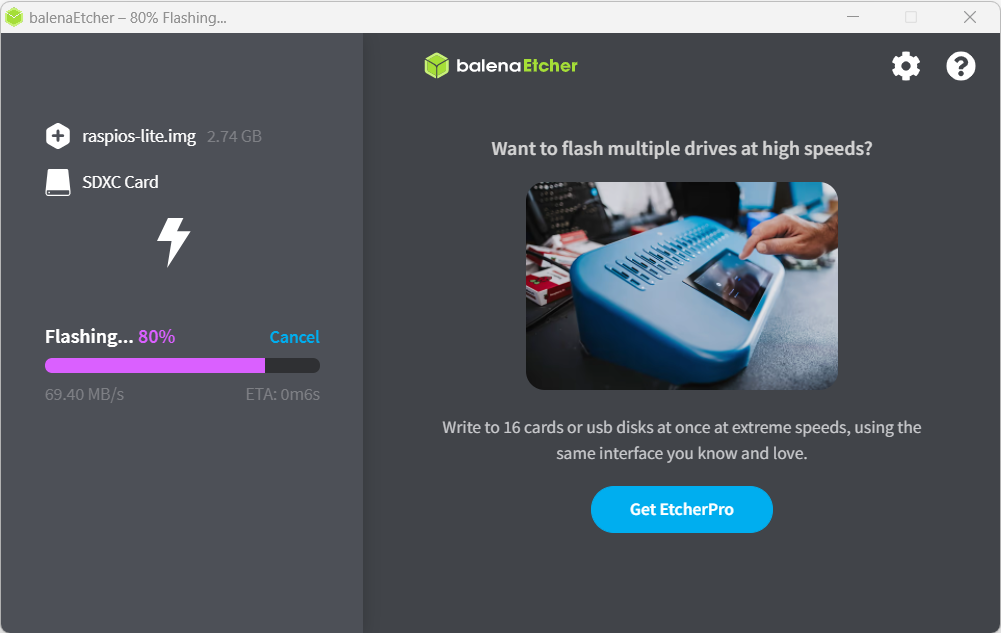
\includegraphics[width=.9\columnwidth]{validation/7_Flashing_SDCard.png}
    \captionof{figure}{\acrshort{os} image flashing}
    \label{fig:7_Flashing_SDCard}
    \endgroup
\end{center}
The Raspberry Pi 4 was then powered up and booted for the first time. All the software was installed and \gls{provisioning} was successfully completed (figure \ref{fig:8_Provisioning_Done}).
\begin{center}
    \begingroup
    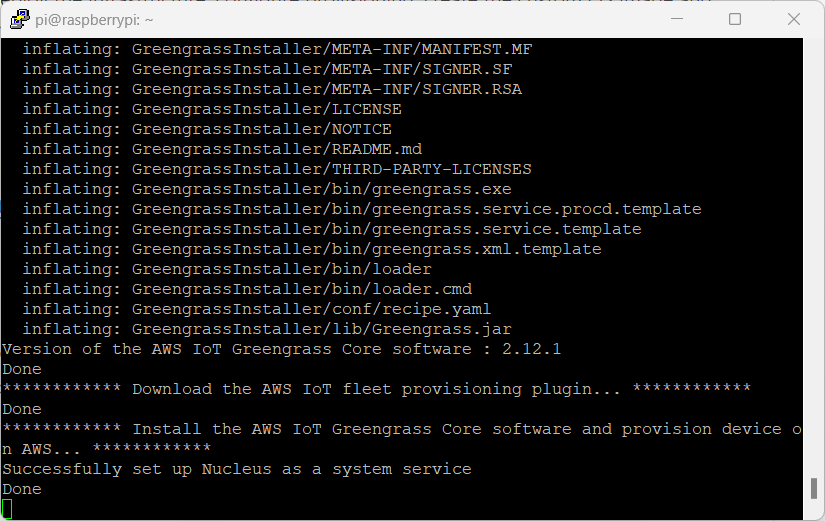
\includegraphics[width=.9\columnwidth]{validation/8_Provisioning_Done.png}
    \captionof{figure}{End of \gls{provisioning} on the device}
    \label{fig:8_Provisioning_Done}
    \endgroup
\end{center}
\Gls{provisioning} is confirmed in figure \ref{fig:8_Provisioned_AWS}. \gls{aws} has created a digital twin of this device on the \gls{aws} \acrshort{iot} service. The name corresponds to its serial number. It is linked to the group created earlier. A unique X.509 certificate has been provided.
\begin{center}
    \begingroup
    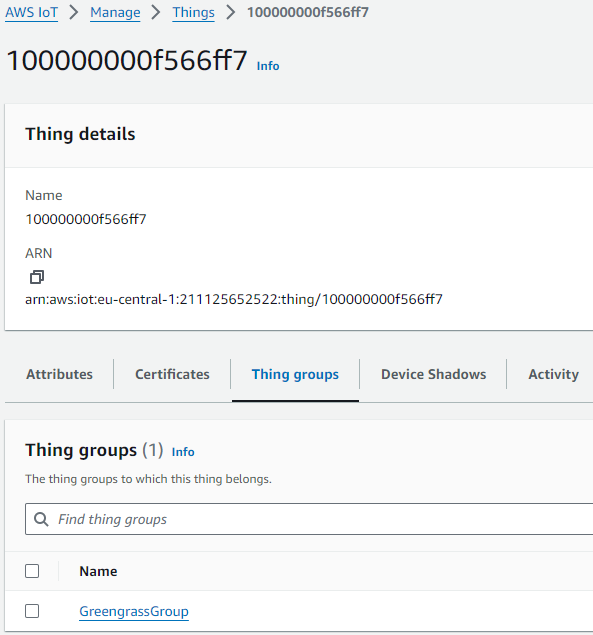
\includegraphics[width=.6\columnwidth]{validation/8_Provisioned_AWS.png}
    \captionof{figure}{Confirmed \gls{provisioning} on \gls{aws}}
    \label{fig:8_Provisioned_AWS}
    \endgroup
\end{center}

\subsection{Adding a second Raspberry Pi 4}
A second Raspberry Pi 4 has been successfully provisioned. Its serial number has been added to the list of authorised devices. A proof of its digital twin can be seen in figure \ref{fig:21_SecondProvisionRPi}.
\begin{center}
    \begingroup
    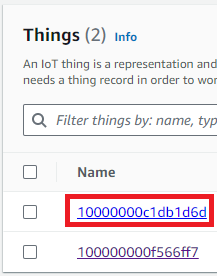
\includegraphics[width=.25\columnwidth]{validation/21_SecondProvisionRPi.png}
    \captionof{figure}{Second provisioning confirmed on \gls{aws}}
    \label{fig:21_SecondProvisionRPi}
    \endgroup
\end{center}
The components have been deployed correctly. A message exchange can be seen on the \gls{aws} \acrshort{mqtt} client interface (figure \ref{fig:21_SecondRPiMQTT}). A new blinking frequency was sent to the second Raspberry Pi 4 and a message from it was returned to \gls{aws} \acrshort{iot}.
\begin{center}
    \begingroup
    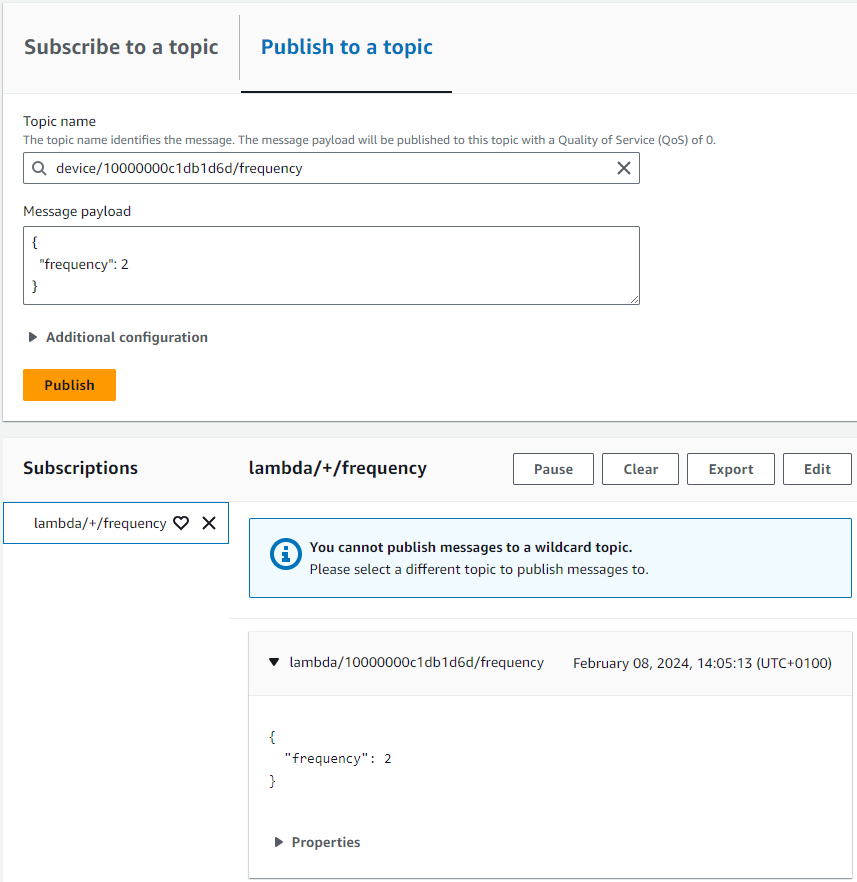
\includegraphics[width=.8\columnwidth]{validation/21_SecondRPiMQTT.png}
    \captionof{figure}{Exchanging \acrshort{mqtt} messages with the second Raspberry Pi 4}
    \label{fig:21_SecondRPiMQTT}
    \endgroup
\end{center}

\section{Applications}

% -- Your text goes here --
All the applications were deployed on the Raspberry Pi 4. As soon as it was provisioned, the deployment started. This can be seen in figure \ref{fig:9_Deployment_InProgress}.
\begin{center}
    \begingroup
    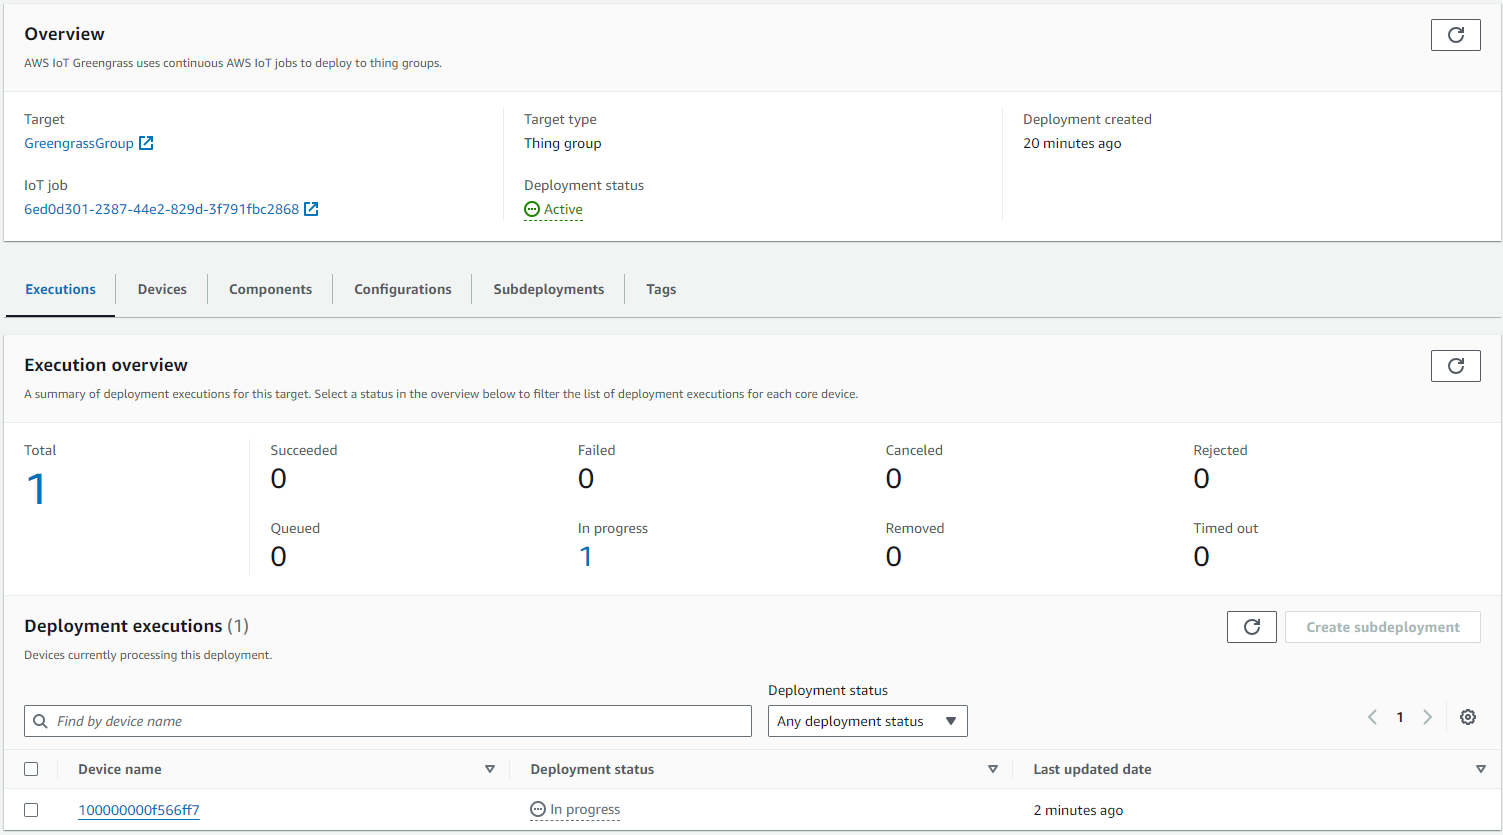
\includegraphics[width=1\columnwidth]{validation/9_Deployment_InProgress.png}
    \captionof{figure}{Deployment of Greengrass components in progress}
    \label{fig:9_Deployment_InProgress}
    \endgroup
\end{center}
Deployment took just a few minutes. The Greengrass components acting as intermediaries for the applications can be seen in figure \ref{fig:11_Components_Running}. The dependencies are also installed in addition to the Greengrass nucleus \textit{aws.greengrass.Nucleus}.
\begin{center}
    \begingroup
    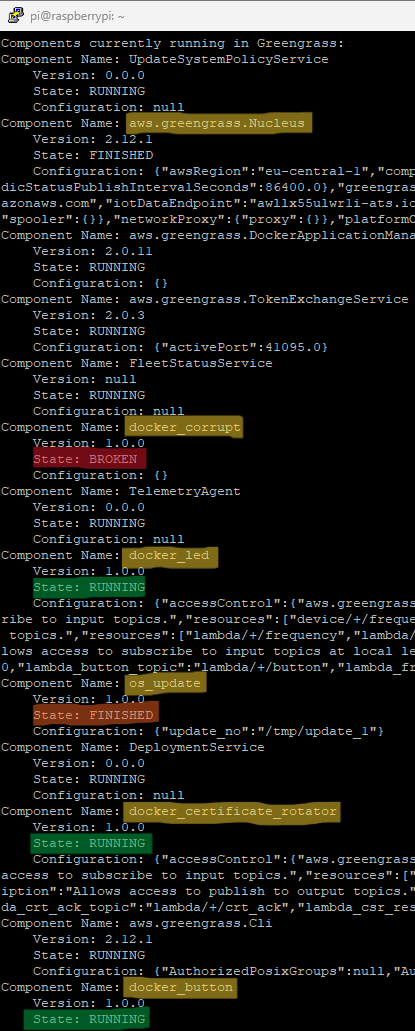
\includegraphics[width=.5\columnwidth]{validation/11_Components_Running.png}
    \captionof{figure}{Greengrass components deployed}
    \label{fig:11_Components_Running}
    \endgroup
\end{center}
It is possible to see an overview of the Raspberry Pi 4 on \gls{aws} as shown in figure \ref{fig:13_DeviceHealth}. Its state of health is poor because a component failed when it was launched. In fact, the corrupted component was unable to start up correctly and was interrupted. The other components are in a state of execution or completion.
\begin{center}
    \begingroup
    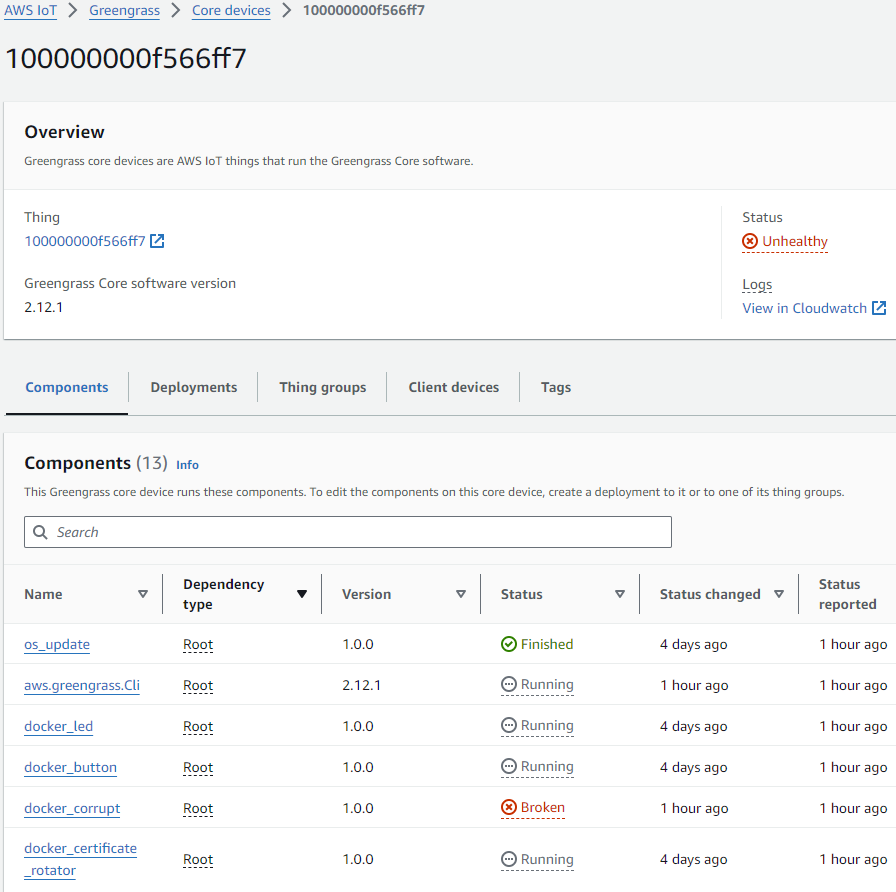
\includegraphics[width=1\columnwidth]{validation/13_DeviceHealth.png}
    \captionof{figure}{Overview of the Raspberry Pi 4 from \gls{aws}}
    \label{fig:13_DeviceHealth}
    \endgroup
\end{center}

\subsection{Applications interaction}
The applications were then tested. The first was the led application. The \gls{aws} web interface was used to send \acrshort{mqtt} messages and view the data received. A message is sent to the Raspberry Pi 4 to change its led blinking frequency. A response was sent back to \gls{aws} \acrshort{iot} in another field including the new frequency. A proof can be found in figure \ref{fig:12_FrequencyChange}.
\begin{center}
    \begingroup
    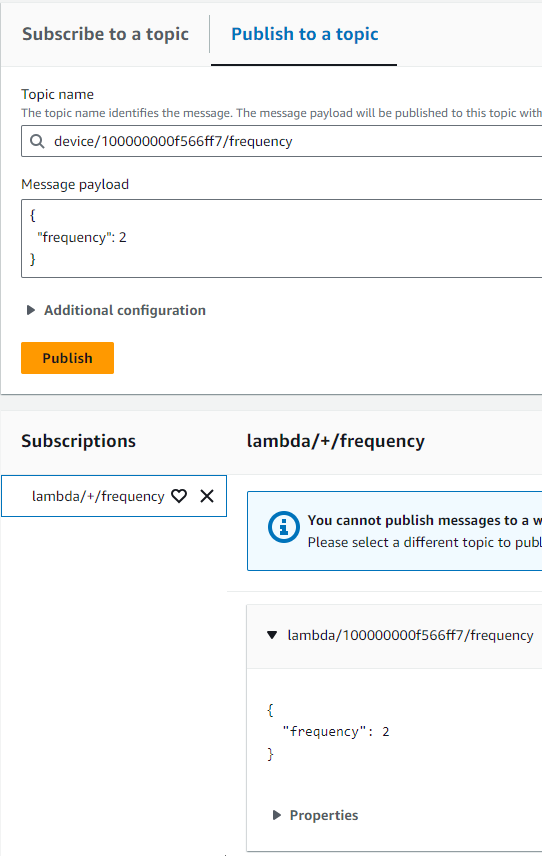
\includegraphics[width=.5\columnwidth]{validation/12_FrequencyChange.png}
    \captionof{figure}{Frequency change on \gls{aws}}
    \label{fig:12_FrequencyChange}
    \endgroup
\end{center}
Figure \ref{fig:12_LedApp_Log} shows the led application output message thread. It is possible to view different frequencies received on the Raspberry Pi 4.
\begin{center}
    \begingroup
    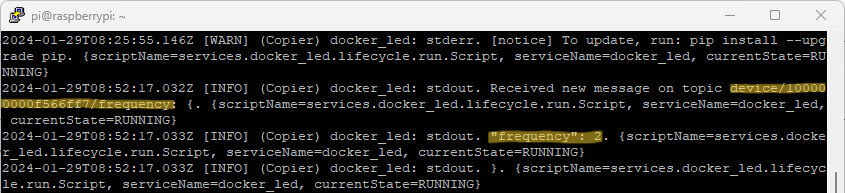
\includegraphics[width=1\columnwidth]{validation/12_LedApp_Log.png}
    \captionof{figure}{Frequency change on the Raspberry Pi 4}
    \label{fig:12_LedApp_Log}
    \endgroup
\end{center}
The button application was also tested. The external button on the Raspberry Pi 4 was pressed twice. \acrshort{mqtt} messages were transmitted to the led application locally and then published to \gls{aws} \acrshort{iot}. The messages can be seen in figure \ref{fig:12_ButtonChange}. The first press deactivates the blinking of the led and the second reactivates it.
\begin{center}
    \begingroup
    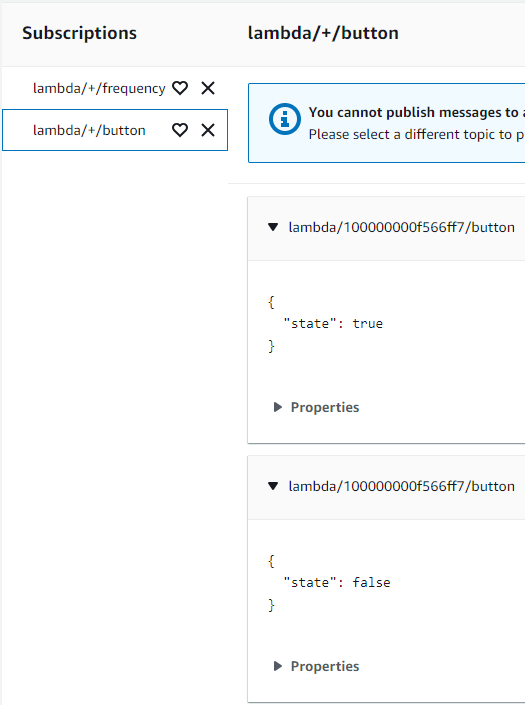
\includegraphics[width=.5\columnwidth]{validation/12_ButtonChange.png}
    \captionof{figure}{Blink status changes on \gls{aws}}
    \label{fig:12_ButtonChange}
    \endgroup
\end{center}
Figure \ref{fig:12_LedApp_Log_button} shows the output message thread of the led application. It is possible to view the \acrshort{mqtt} messages received from the button application on the Raspberry Pi 4.
\begin{center}
    \begingroup
    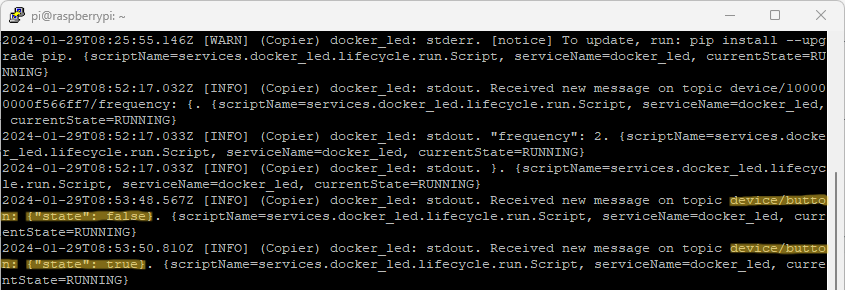
\includegraphics[width=1\columnwidth]{validation/12_LedApp_Log_button.png}
    \captionof{figure}{Blink status changes on the Raspberry Pi 4}
    \label{fig:12_LedApp_Log_button}
    \endgroup
\end{center}
Finally, the certificate was rotated. The triggering of a change alert was simulated from the \gls{aws} \acrshort{mqtt} interface by requesting the creation of \acrshort{csr} on the Raspberry Pi 4. Several \acrshort{mqtt} messages were exchanged. These are partly visible from the \gls{aws} interface in figure \ref{fig:12_CertRotate}. When analysing the digital twin, the certificate identifier was changed, proving that the rotation had indeed taken place. The Greengrass service was also restarted to take the new certificate into account.
\begin{center}
    \begingroup
    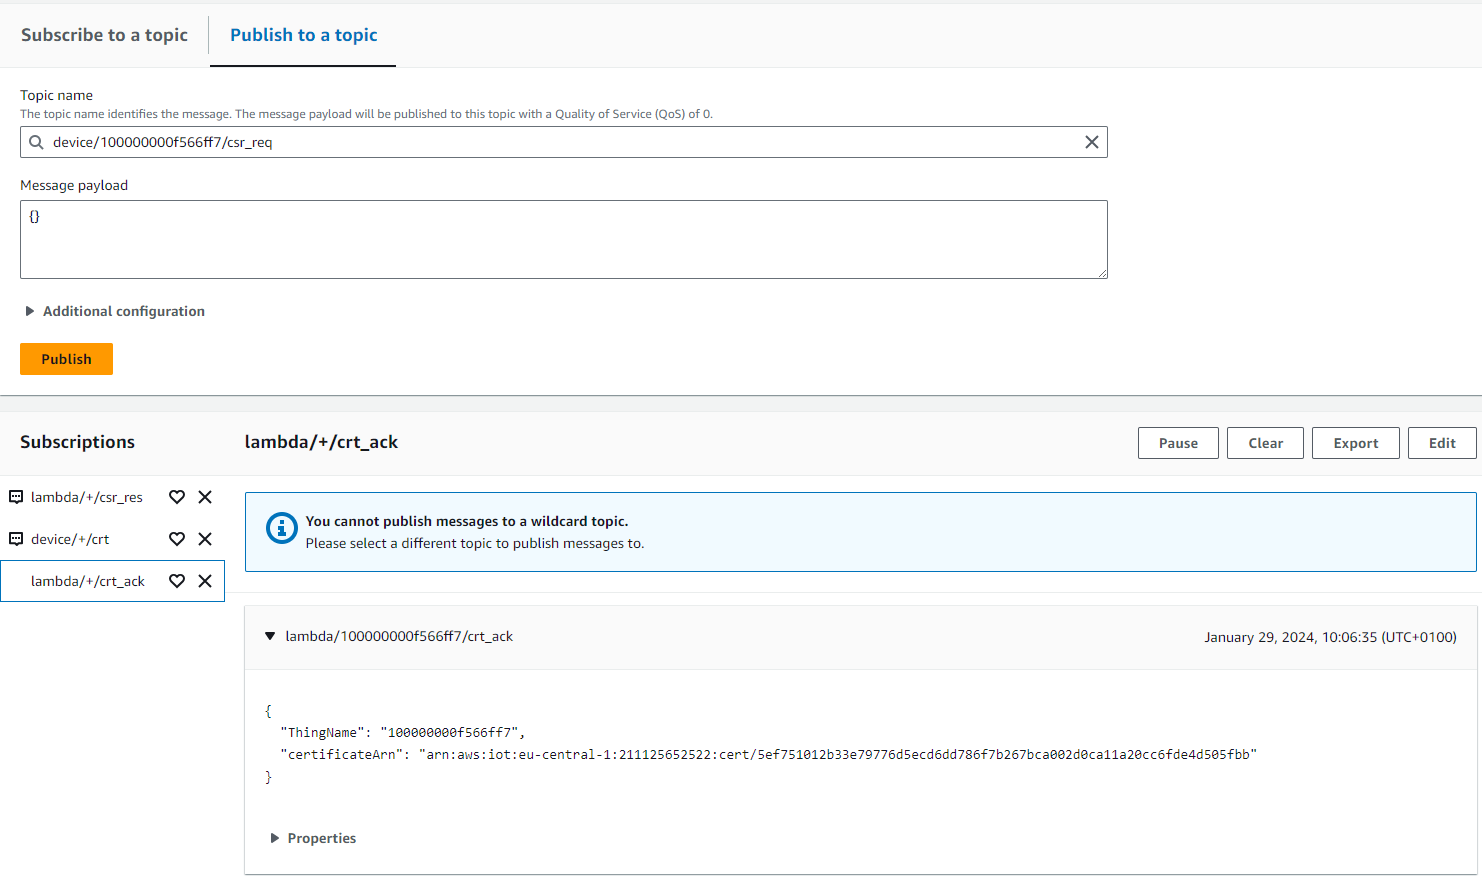
\includegraphics[width=1\columnwidth]{validation/12_CertRotate.png}
    \captionof{figure}{Certificate rotation on \gls{aws}}
    \label{fig:12_CertRotate}
    \endgroup
\end{center}
Figure \ref{fig:12_CertRotate_Log} shows the output message thread of the certificate rotation application. It is possible to view the \acrshort{mqtt} messages received from \gls{aws}. A request for \acrshort{csr} has been received as well as the new certificate.
\begin{center}
    \begingroup
    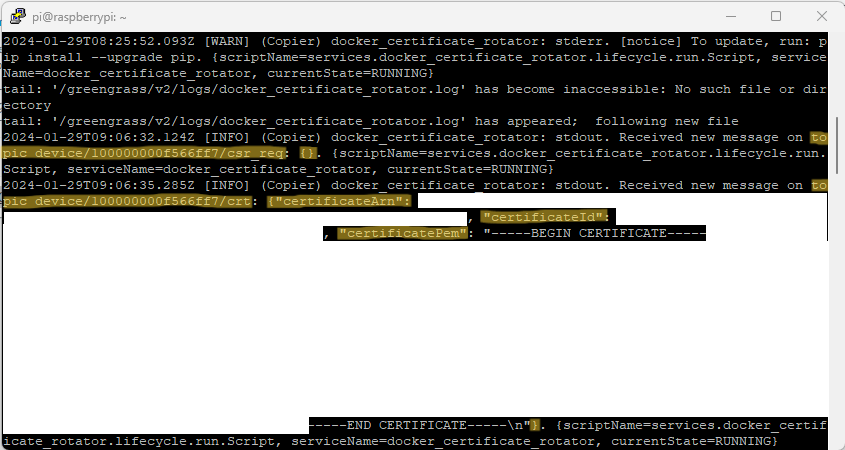
\includegraphics[width=1\columnwidth]{validation/12_CertRotate_Log.png}
    \captionof{figure}{Certificate rotation on the Raspberry Pi 4}
    \label{fig:12_CertRotate_Log}
    \endgroup
\end{center}
Due to the incorrect platform specified for the corrupted application, it was unable to start up correctly. This is clearly shown in figure \ref{fig:12_CorruptApp_Log}. Greengrass tries to start the application three times before stopping.
\begin{center}
    \begingroup
    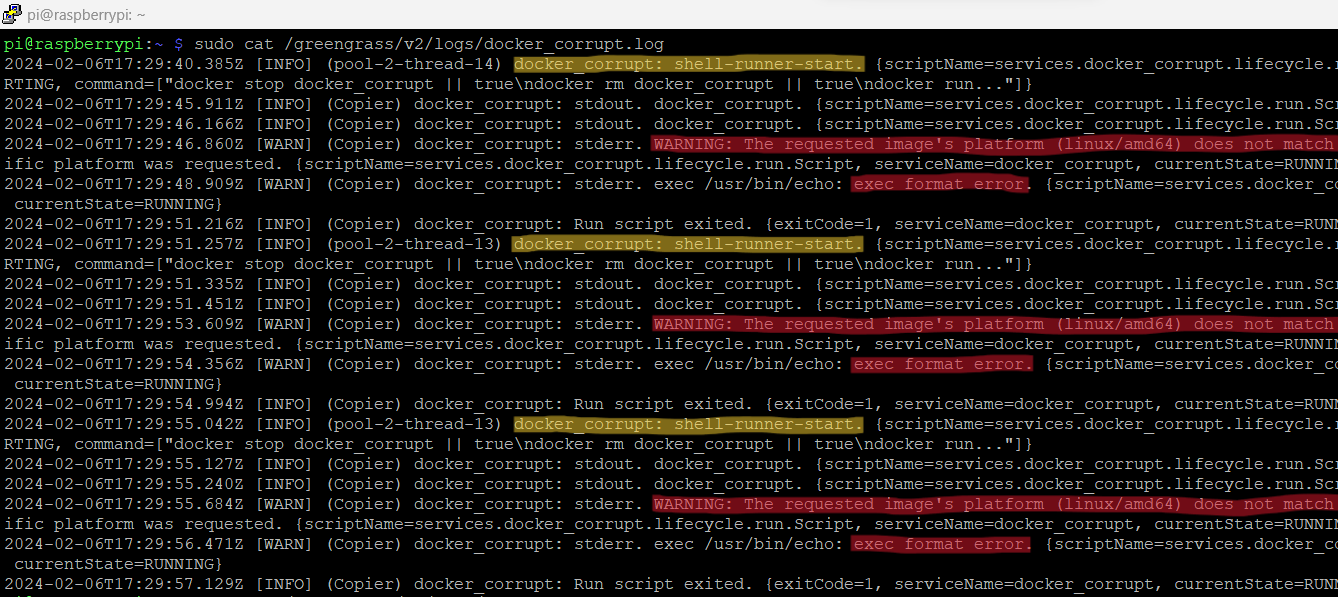
\includegraphics[width=1\columnwidth]{validation/12_CorruptApp_Log.png}
    \captionof{figure}{Launching the corrupt application on the Raspberry Pi 4}
    \label{fig:12_CorruptApp_Log}
    \endgroup
\end{center}
During testing of the components, an additional observation was made. If a component is corrupted and subsequently deployed with updates to other components, these components will retain the old version. As long as the corrupted application is not corrected, all the components remain frozen on the last version deployed, and not on the last version of the component.

\subsection{Updating an application}
In order to test the deployment of an update, the corrupted application was corrected by specifying the correct architecture. The Greengrass component has been updated since it has changed version (figure \ref{fig:14_NewComponentVersion}).
\begin{center}
    \begingroup
    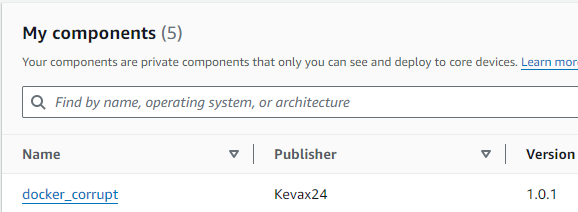
\includegraphics[width=.8\columnwidth]{validation/14_NewComponentVersion.png}
    \captionof{figure}{New version of the corrupted application on \gls{aws}}
    \label{fig:14_NewComponentVersion}
    \endgroup
\end{center}
Looking at the Raspberry Pi 4 console in figure \ref{fig:14_CorruptApp_updated}, the application ran correctly. A text was printed as agreed.
\begin{center}
    \begingroup
    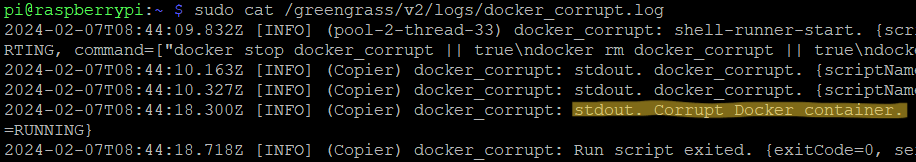
\includegraphics[width=1\columnwidth]{validation/14_CorruptApp_updated.png}
    \captionof{figure}{Preview of the corrupted application on the Raspberry Pi 4}
    \label{fig:14_CorruptApp_updated}
    \endgroup
\end{center}
Now that no components have been corrupted, the health of the \acrshort{iot} device is good. This was noted on the \gls{aws} console.

\subsection{\texorpdfstring{\acrshort{os}}{} update}
An update simulation was tested. The commands written were executed correctly and the Raspberry Pi 4 rebooted automatically without restarting the command lines. Evidence of this can be seen in figure \ref{fig:20_os_update}. The first time it was run, the \textit{apt-get update} command was issued, followed by the restart command. When the Greengrass component is launched a second time, it is noted that the update has already taken place.
\begin{center}
    \begingroup
    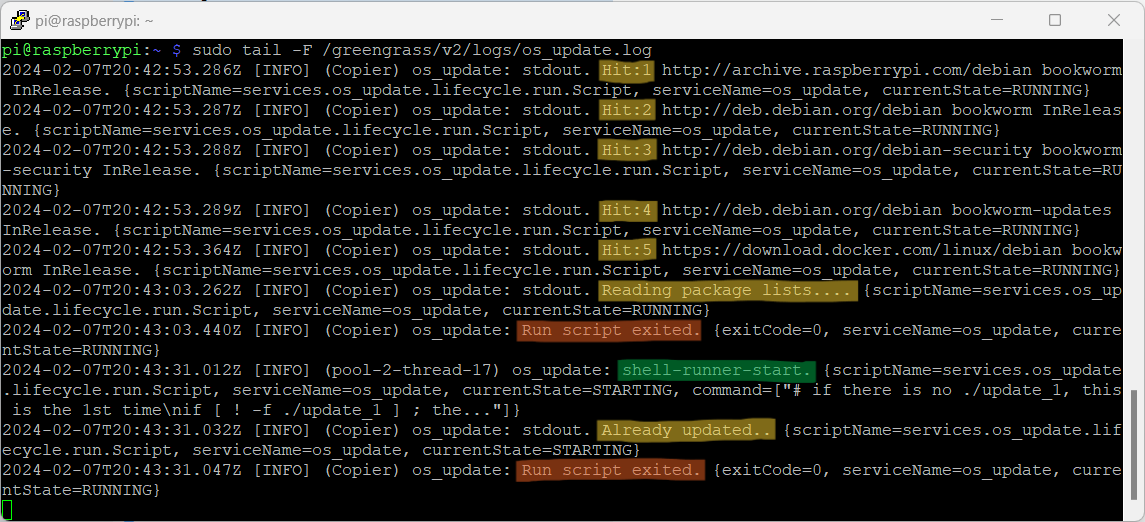
\includegraphics[width=1\columnwidth]{validation/20_os_update.png}
    \captionof{figure}{Behaviour of the \acrshort{os} update application}
    \label{fig:20_os_update}
    \endgroup
\end{center}

\section{\texorpdfstring{\Gls{cloud_infrastructure}}{} destruction}

% -- Your text goes here --
The \gls{cloud_infrastructure} destruction was tested. To do this, the corresponding workflow was launched manually from the GitHub Actions console and passed successfully (figure \ref{fig:15_DestroyInfra}). It takes about 4 minutes. All the resources created by the Pulumi tool have been deleted. The Raspberry Pi 4 remains provisioned with its unique certificate. The claim certificate remains available in the S3 bucket with its private key. The Greengrass components have not been removed either.
\begin{center}
    \begingroup
    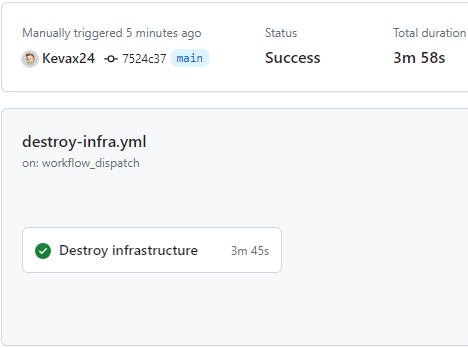
\includegraphics[width=.6\columnwidth]{validation/15_DestroyInfra.png}
    \captionof{figure}{\Gls{cloud_infrastructure} destruction successfully completed}
    \label{fig:15_DestroyInfra}
    \endgroup
\end{center}
The Raspberry Pi 4's digital twin is still contained within \gls{aws} \acrshort{iot}. However, it has lost any policy for interacting with the \gls{cloud}. The \acrshort{mqtt} connection is therefore interrupted except locally on the device between the components. This was proven by pressing the external button on the Raspberry Pi 4 just once. The led stopped blinking and no status message was received on \gls{aws} \acrshort{iot}.

\section{Management of authorised embedded systems}

% -- Your text goes here --
\subsection{Infrastructure deployment with a provisioned embedded system}
Following the logic of the tests, the infrastructure was redeployed with the Raspberry Pi 4 already provisioned. Its digital twin was attached to the group of devices and to an \acrshort{iot} policy. \acrshort{mqtt} communication with the \gls{cloud} is now back up and running. Figure \ref{fig:16_AttachExistingThing} shows the attachment of the device to the new \gls{cloud_infrastructure} in the GitHub Actions console.
\begin{center}
    \begingroup
    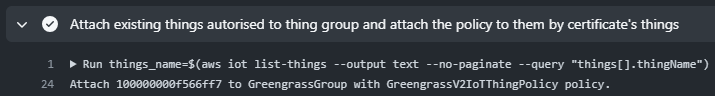
\includegraphics[width=1\columnwidth]{validation/16_AttachExistingThing.png}
    \captionof{figure}{Integration of Raspberry Pi 4 already provisioned}
    \label{fig:16_AttachExistingThing}
    \endgroup
\end{center}

\subsection{Deleting a provisioned embedded system}
It is possible to remove a device from the \gls{aws} \gls{cloud} by deleting its serial number from the list of authorised devices. The serial number of the provisioned Raspberry Pi 4 has therefore been removed and this change has been pushed into Git. By following the GitHub Actions console in figure \ref{fig:17_RemoveThing}, it is possible to confirm that the device has been deleted. By browsing the \gls{aws} console, its digital twin no longer exists and no \acrshort{mqtt} message reaches \gls{aws} \acrshort{iot}.
\begin{center}
    \begingroup
    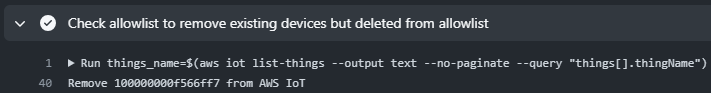
\includegraphics[width=1\columnwidth]{validation/17_RemoveThing.png}
    \captionof{figure}{Removal of the provisioned Raspberry Pi 4}
    \label{fig:17_RemoveThing}
    \endgroup
\end{center}
For this Raspberry Pi 4 to be provisioned again, it must be authorised again and its SD card must be flashed again with the \acrshort{os} image.

\subsection{Unauthorised provisioning of an embedded system}
This same Raspberry Pi 4 was tested for reintegration into the \gls{cloud_infrastructure} without being authorised. Its serial number was therefore not included in the list of authorised devices. Its SD card was flashed with the same \acrshort{os} image as for all the other tests carried out. Both software, Docker Engine and \gls{aws} \acrshort{iot} Greengrass, were successfully installed. During the provisioning attempt, the Lambda function, triggered at each attempt, detected that this Raspberry Pi 4 was not authorised to be provisioned. Its certificate, which had been prepared and was supposed to be delivered to it, was therefore left waiting to be activated. After a while, the certificate disappears. This can be seen in figure \ref{fig:18_CertificatPending}.
\begin{center}
    \begingroup
    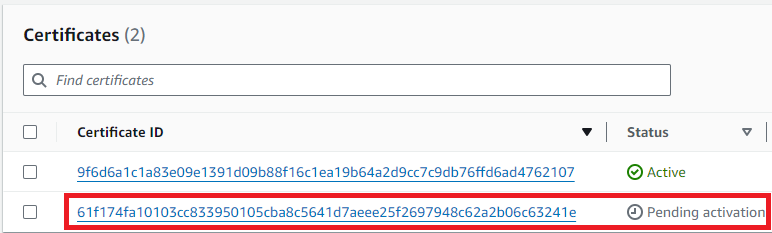
\includegraphics[width=1\columnwidth]{validation/18_CertificatPending.png}
    \captionof{figure}{Certificat en attente d'activation}
    \label{fig:18_CertificatPending}
    \endgroup
\end{center}

\section{Provisioning of other Arm SystemReady certified embedded systems}

% -- Your text goes here --

\section{\texorpdfstring{\Gls{cloud_infrastructure}}{} cost}

% -- Your text goes here --
An assessment of the costs of the \gls{aws} \gls{cloud_infrastructure} was carried out in order to understand the monthly and annual expenses to be expected. This estimate was carried out using the \gls{aws} Pricing Calculator. The estimate is shown in figure \ref{fig:19_CostEstimate}.
\begin{center}
    \begingroup
    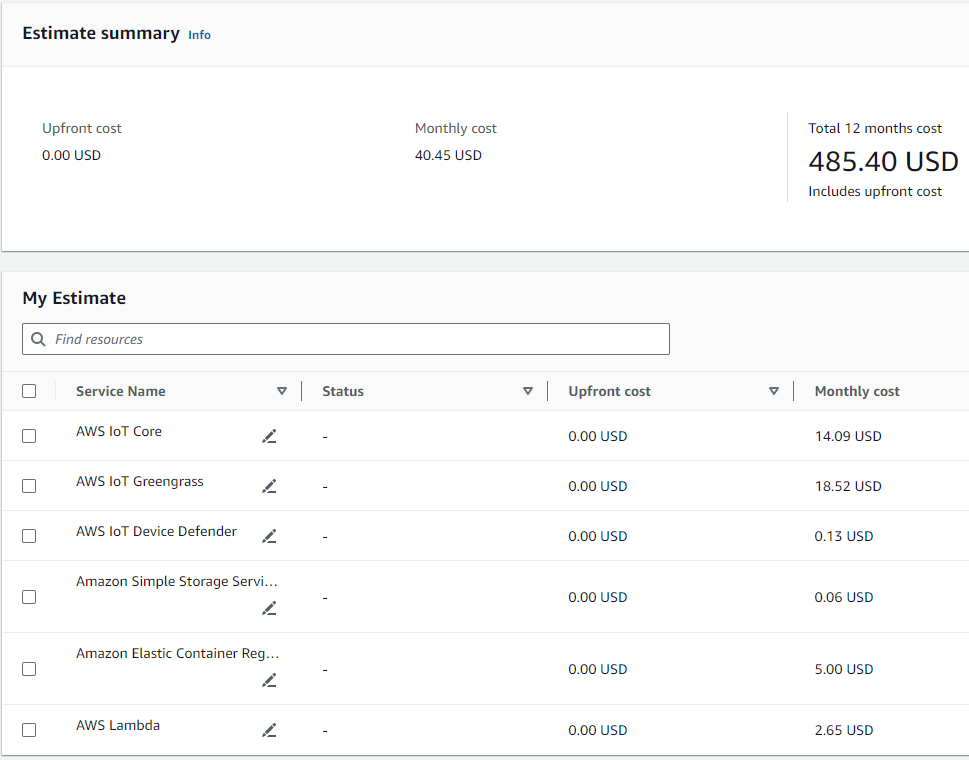
\includegraphics[width=1\columnwidth]{validation/19_CostEstimate.png}
    \captionof{figure}{\Gls{cloud_infrastructure} cost estimate}
    \label{fig:19_CostEstimate}
    \endgroup
\end{center}
The evaluation is based on a number of factors, assuming that it is the cost of the infrastructure in the production environment. The region chosen is Frankfurt (\textit{eu-central-1}). A fleet of 100 embedded systems is considered.

\gls{aws} \acrshort{iot} Core is a high-cost service. Here is a list of factors taken into account :
\begin{itemize}
    \item Number of devices : 100
    \item Protocol : \acrshort{mqtt}
    \item Average size per message : 10 kB
    \item Number of messages per month per device : 43'800 (1 par minute)
    \item Number of rules triggered per month per device : 43'800
\end{itemize}
Each device sends one 10 kB \acrshort{mqtt} message per minute. Each message received in \gls{aws} \acrshort{iot} Core triggers a rule that diverts the message to another service. For example, Lambda functions can be called by these rules depending on the message heading.

\gls{aws} \acrshort{iot} Greengrass is the most expensive service. Here are the factors taken into consideration:
\begin{itemize}
    \item Number of devices : 100
    \item Activity period per month : 43'800 minutes (100\% activity)
    \item Number of \acrshort{mqtt} topics : 1000
\end{itemize}
With 1000 \acrshort{mqtt} topics, each device can have 10 unique topics each.

The \gls{aws} \acrshort{iot} Device Defender service is used to perform a daily audit by monitoring a single aspect, namely the expiry of certificates. The cost is virtually insignificant.

The \gls{aws} Lambda service is used to execute operations when a function is triggered by a received message. It is estimated that each message received triggers a function, with a total of 4''380'000 messages sent per month for the fleet of 100 embedded systems. The average execution time for a Lambda function is one second.

Amazon \acrfull{ecr} is used to store the Docker images generated for the applications developed. A monthly storage limit of 50 GB has been defined. None of the application images in this project exceeds 400 MB. Therefore, there can be up to 125 images of this size to reach the 50 GB limit.

Amazon S3 is also used for storage, with three S3 buckets in use. The bucket containing the OS image for this reference architecture weighs 2.6 GB. The total of the three buckets remains at 2.6 GB, indicating that the Pulumi files on the state of the infrastructure, in addition to the provisioning files, do not exceed 100 MB.

The Amazon SNS service used in the reference architecture is not taken into account, as it is triggered every so many years (a certificate has a lifetime of several years by default). Consequently, its cost is negligible.